\documentclass{article}
\usepackage{amsmath}
\usepackage{amssymb}
\usepackage{graphicx}
\usepackage{hyperref}
\usepackage{enumitem}
\usepackage{times}
\usepackage{breqn}
\usepackage{fancyhdr,graphicx,amsmath,amssymb}
\usepackage[ruled,vlined]{algorithm2e}
\usepackage{tikz-qtree}
\usepackage{tikz}
\include{pythonlisting}
\usetikzlibrary{shapes,arrows,backgrounds,positioning}

\tikzset{
  treenode/.style = {align=center, inner sep=0pt, text centered,
    font=\sffamily},
  arn_n/.style = {treenode, circle, black, font=\sffamily\bfseries, draw=black,
    fill=white, text width=1.5em},% arbre rouge noir, noeud noir
  arn_r/.style = {treenode, circle, red, draw=red, 
    text width=1.5em, very thick},% arbre rouge noir, noeud rouge
  arn_x/.style = {treenode, rectangle, draw=black,
    minimum width=0.5em, minimum height=0.5em}% arbre rouge noir, nil
}

\title{Algorithms Homework 5}
\author{Koi Stephanos}
\date{October 2019}

\begin{document}

\maketitle

\begin{enumerate}
\item
    MergeSort, QuickSort and HeapSort are all sorting algorithms of the class \(O(nlgn)\), but have unique characteristics which gives each advantages and disadvantages when considering data size and status as well as operating constraints. 
    
    MergeSort works best with chunks of data that are already sorted, and is the best choice of the three in that case, but does require more memory, as a second array must be created for the merges. Quicksort has the slowest worst case at \(O(n^2)\), but doesn't require extra memory, but unlike MergeSort, is massively recursive. As long as a pivot point is chosen randomely, and the data isn't sorted, QuickSort is a good option for both speed and memory and is often the default sorting algorithm as a result. HeapSort in some ways offers a compromise. An efficient HeapSort, provided the heap fits entirely in memory, does not require extra memory like MergeSort or massive recursion like QuickSort, but unfortunatley is frequently outperformed by both. 
\item
   \begin{enumerate}[label=(\alph*)]
        \item Unsorted Array
        \\[\medskipamount]
            Search: \(O(n)\)
            \\Insert: \(O(1)\)
            \\Delete: \(O(n)\)
            
        \item Sorted Array
        \\[\medskipamount]
        Search:	\(O(log n)\)
        \\Insert:	\(O(n)\)
        \\Delete:	\(O(n)\)
        
        \item Linked List
        \\[\medskipamount]
        Search:	\(O(n)\)
        \\Insert:	\(O(1)\)
        \\Delete:	\(O(1)\)
        
        \item Hash
        \\[\medskipamount]
        Search:	\(O(n)\)
        \\Insert:	\(O(n)\)
        \\Delete:	\(O(n)\)
        
        \pagebreak
        \item Stack
        \\[\medskipamount]
        Search:	\(O(n)\)
        \\Insert:	\(O(1)\)
        \\Delete:	\(O(1)\)
        
        \item Queue
        \\[\medskipamount]
        Search:	\(O(n)\)
        \\Insert:	\(O(1)\)
        \\Delete:	\(O(1)\)
        
        \item Heap
        \\[\medskipamount]
        Search:	\(O(n)\)
        \\Insert:	\(O(lg n)\)
        \\Delete:	\(O(lg n)\)
        
        \item Binomial Heap
        \\[\medskipamount]
        Search:	\(O(n)\)
        \\Insert:	\(O(1)\)
        \\Delete:	\(O(lg n)\)
        
        \item Fibonacci Heap
        \\[\medskipamount]
        Search:	\(O(n)\)
        \\Insert:	\(O(1)\)
        \\Delete:	\(O(lg n)\)

    \end{enumerate}
    
\item 
    A self-balancing binary search tree is a tree in which each node can have at most two children, and whenever inserts and deletes are performed, the tree is re-balanced to minimize the total height. As a result, navigating the tree can consistently be done in \(O(lgn)\) time. Since these properties are inherently abstract, there are multiple ways in which such a tree can be implemented, such as:
    
    \begin{enumerate}[label=(\alph*)]
        \item AVL Tree
        \\[\medskipamount]
            A binary search tree is an AVL Tree iff the difference between the heights of the left and right size are at most 1. In other words, the left and right sides of our tree must be as balanced as possible. This means that the total height of our tree is kept to at most \(lgn\), because each level of the tree has at most \(2^k\) nodes, where \(k\) is the level of the tree. 
        \item Red-Black Tree
        \\[\medskipamount]
            This implementation is very similar to the AVL tree, and has the same goal of maintaining the height of the tree. Here, however, instead of only being concerned about height, we also assign a red or black value to each node, beginning with black for the root. Here, no node can have children of the same color. This results in a less balanced tree than AVL, and as a result, a slower search time, but incurs less overhead for inserts and deletes, because the re-balancing is less expensive, making it a better fit for situations in which you are frequently making changes to the contents of the tree.
        \item Splay Tree
        \\[\medskipamount]
            A Splay Tree operates a bit differently, but has the same fundamental goals of minimizing tree height upon insertions and deletions, but has the extra component of restructuring the tree such that the most recently accessed node then becomes the root of the tree. This works much like the principal of locality, in that you are more likely to need something if you recently need that thing. This means that look up times will improve dramatically if searching for a recently used item, making it a good choice in situations like that, but does add significant overhead as every look up requires a re-balancing. 
        
    \end{enumerate}

\item
    A priority queue implemented with a heap essentially mirrors our MaxHeap lab, in which the heap is represented as an array starting at index 1 and for any node, \(A[k]\), its left child is \(A[k*2]\), and its right child is \(A[k*2 + 1]\). Here, priority is defined as a greater value, such that \(2\) takes priority over \(1\). 
    
    Extracting the next element from the queue equates to extracting the max and then rebalancing the heap. To insert, we place our new value at the end of the array, and then walk it up the heap until it is less than or equal to its parent. In this way, a duplicate value inserted will rise until it is equal in priority to its parent, at which point the fact its parent was in the heap first takes precedence.


\item \leavevmode\vadjust{\vspace{-\baselineskip}}\newline
The Fibonacci Heap after extracting the min:
    \begin{center}
    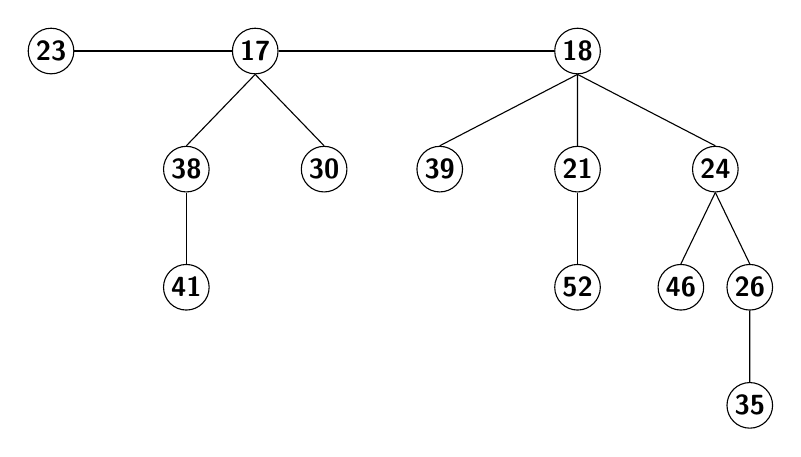
\begin{tikzpicture}[-,>=stealth',level/.style={sibling distance = 1.75cm/#1,level distance = 1.5cm}]
    \node [arn_n](A) {23};
    \node [arn_n, right= 2cm of A](B) {17}
        child{ node [arn_n] {38}
                child{ node [arn_n] {41} 
                }
    		}
    	child{ node [arn_n] {30}  }
    ;
    \node [arn_n, right= 3.5cm of B](C){18}
        child{ node [arn_n] {39}  }
        child{ node [arn_n] {21}
                child{ node [arn_n] {52} 
                }
    		}
    	child{ node [arn_n] {24}
                child{ node [arn_n] {46} 
                }
                child{ node [arn_n] {26}
    							child{ node [arn_n] {35}}
                }
    		}
    ;
    \draw (A) -- (B);
    \draw (B) -- (C);
    \end{tikzpicture}
    \end{center}
    
\pagebreak
\item
    \begin{enumerate}[label=(\alph*)]
    \setlength\itemsep{4em}
    
    \item \leavevmode\vadjust{\vspace{-\baselineskip}}\newline
        \begin{center}
        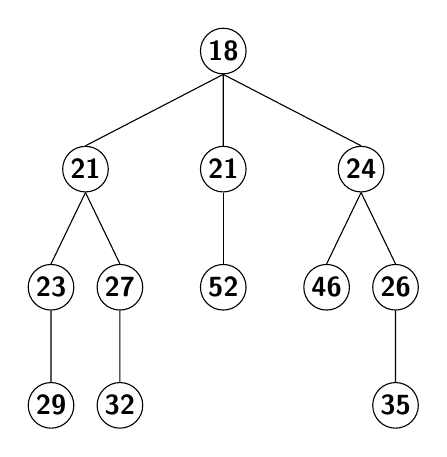
\begin{tikzpicture}[-,>=stealth',level/.style={sibling distance = 1.75cm/#1,level distance = 1.5cm}]
        \node [arn_n](A){18}
            child{ node [arn_n] {21} 
                child{ node [arn_n] {23} 
                    child{ node [arn_n] {29}}
                }
                    child{ node [arn_n] {27}
                        child{ node [arn_n] {32}}
        		}		
            }
            child{ node [arn_n] {21}
                    child{ node [arn_n] {52} 
                    }
        		}
        	child{ node [arn_n] {24}
                    child{ node [arn_n] {46} 
                    }
                    child{ node [arn_n] {26}
        							child{ node [arn_n] {35}}
                    }
        		}
        ;
        \end{tikzpicture}
        \end{center}
    
    \item \leavevmode\vadjust{\vspace{-\baselineskip}}\newline
        \begin{center}
        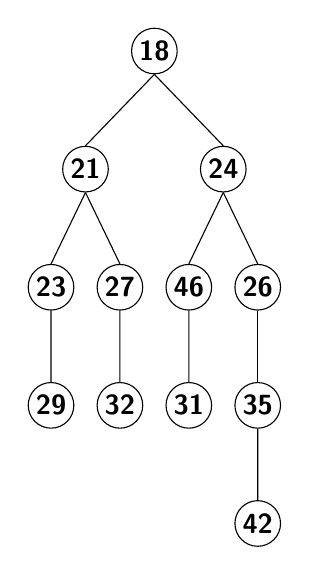
\begin{tikzpicture}[-,>=stealth',level/.style={sibling distance = 1.75cm/#1,level distance = 1.5cm}]
        \node [arn_n](A){18}
            child{ node [arn_n] {21} 
                child{ node [arn_n] {23} 
                    child{ node [arn_n] {29}}
                }
                    child{ node [arn_n] {27}
                        child{ node [arn_n] {32}}
        		}		
            }
        	child{ node [arn_n] {24}
                    child{ node [arn_n] {46} 
                        child{ node [arn_n] {31}}
                    }
                    child{ node [arn_n] {26}
        							child{ node [arn_n] {35}
        							    child{ node [arn_n] {42}}
        				}
                    }
        		}
        ;
        \end{tikzpicture}
        \end{center}
\pagebreak
    \item \leavevmode\vadjust{\vspace{-\baselineskip}}\newline
        \begin{center}
        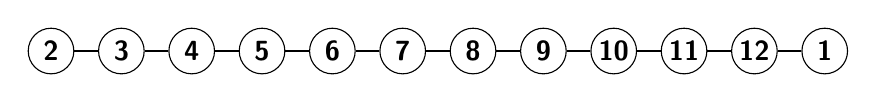
\begin{tikzpicture}[-,>=stealth',level/.style={sibling distance = 1.75cm/#1,level distance = 1.5cm}]
        \node [arn_n](A){2};
        \node [arn_n, right= .3cm of A](B){3};
        \node [arn_n, right= .3cm of B](C){4};
        \node [arn_n, right= .3cm of C](D){5};
        \node [arn_n, right= .3cm of D](E){6};
        \node [arn_n, right= .3cm of E](F){7};
        \node [arn_n, right= .3cm of F](G){8};
        \node [arn_n, right= .3cm of G](H){9};
        \node [arn_n, right= .3cm of H](I){10};
        \node [arn_n, right= .3cm of I](J){11};
        \node [arn_n, right= .3cm of J](K){12};
        \node [arn_n, right= .3cm of K](L){1};
        
        \draw (A) -- (B);
        \draw (B) -- (C);
        \draw (C) -- (D);
        \draw (D) -- (E);
        \draw (E) -- (F);
        \draw (F) -- (G);
        \draw (G) -- (H);
        \draw (H) -- (I);
        \draw (I) -- (J);
        \draw (J) -- (K);
        \draw (K) -- (L);

        \end{tikzpicture}
        \end{center}
        
    \item \leavevmode\vadjust{\vspace{-\baselineskip}}\newline
        \begin{center}
        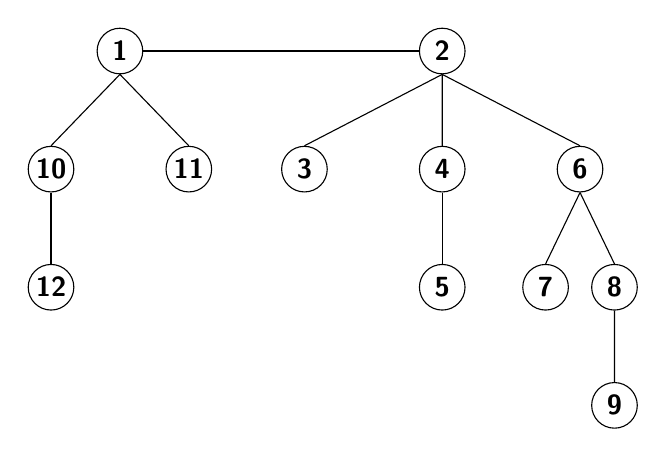
\begin{tikzpicture}[-,>=stealth',level/.style={sibling distance = 1.75cm/#1,level distance = 1.5cm}]
        \node [arn_n](A) {1}
            child{ node [arn_n] {10}
                    child{ node [arn_n] {12} 
                    }
        		}
        	child{ node [arn_n] {11}  }
        ;
        \node [arn_n, right= 3.5cm of A](B){2}
            child{ node [arn_n] {3}  }
            child{ node [arn_n] {4}
                    child{ node [arn_n] {5} 
                    }
        		}
        	child{ node [arn_n] {6}
                    child{ node [arn_n] {7} 
                    }
                    child{ node [arn_n] {8}
        							child{ node [arn_n] {9}}
                    }
        		}
        ;
        \draw (A) -- (B);
        \end{tikzpicture}
        \end{center}
    
    \end{enumerate}
    
\item
    \begin{enumerate}[label=(\alph*)]
    \setlength\itemsep{4em}
    
    \item \leavevmode\vadjust{\vspace{-\baselineskip}}\newline
        \begin{center}
        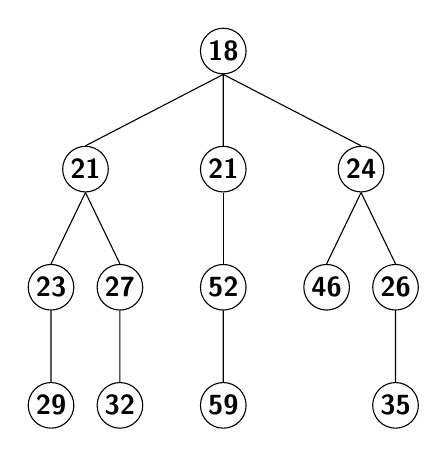
\begin{tikzpicture}[-,>=stealth',level/.style={sibling distance = 1.75cm/#1,level distance = 1.5cm}]
        \node [arn_n](A){18}
            child{ node [arn_n] {21} 
                child{ node [arn_n] {23} 
                    child{ node [arn_n] {29}}
                }
                    child{ node [arn_n] {27}
                        child{ node [arn_n] {32}}
        		}		
            }
            child{ node [arn_n] {21}
                    child{ node [arn_n] {52} 
                        child{ node [arn_n] {59}}
                    }
        		}
        	child{ node [arn_n] {24}
                    child{ node [arn_n] {46} 
                    }
                    child{ node [arn_n] {26}
        							child{ node [arn_n] {35}}
                    }
        		}
        ;
        \end{tikzpicture}
        \end{center}
\pagebreak    
    \item \leavevmode\vadjust{\vspace{-\baselineskip}}\newline
        \begin{center}
        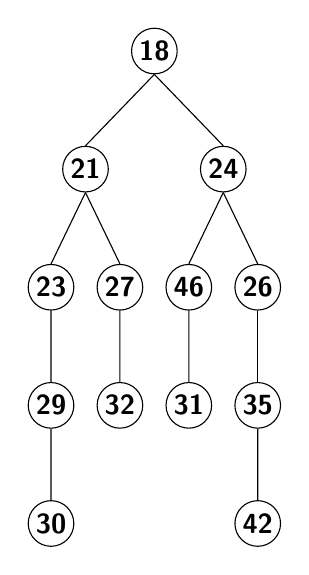
\begin{tikzpicture}[-,>=stealth',level/.style={sibling distance = 1.75cm/#1,level distance = 1.5cm}]
        \node [arn_n](A){18}
            child{ node [arn_n] {21} 
                child{ node [arn_n] {23} 
                    child{ node [arn_n] {29}
                        child{ node [arn_n] {30}}
                    }
                }
                    child{ node [arn_n] {27}
                        child{ node [arn_n] {32}}
        		}		
            }
        	child{ node [arn_n] {24}
                    child{ node [arn_n] {46} 
                        child{ node [arn_n] {31}}
                    }
                    child{ node [arn_n] {26}
        							child{ node [arn_n] {35}
        							    child{ node [arn_n] {42}}
        				}
                    }
        		}
        ;
        \end{tikzpicture}
        \end{center}

    \item \leavevmode\vadjust{\vspace{-\baselineskip}}\newline
        \begin{center}
        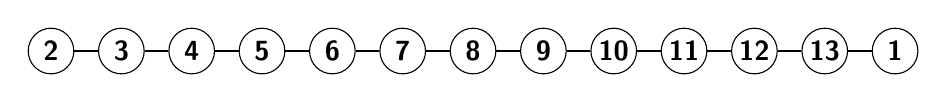
\begin{tikzpicture}[-,>=stealth',level/.style={sibling distance = 1.75cm/#1,level distance = 1.5cm}]
        \node [arn_n](A){2};
        \node [arn_n, right= .3cm of A](B){3};
        \node [arn_n, right= .3cm of B](C){4};
        \node [arn_n, right= .3cm of C](D){5};
        \node [arn_n, right= .3cm of D](E){6};
        \node [arn_n, right= .3cm of E](F){7};
        \node [arn_n, right= .3cm of F](G){8};
        \node [arn_n, right= .3cm of G](H){9};
        \node [arn_n, right= .3cm of H](I){10};
        \node [arn_n, right= .3cm of I](J){11};
        \node [arn_n, right= .3cm of J](K){12};
        \node [arn_n, right= .3cm of K](L){13};
        \node [arn_n, right= .3cm of L](M){1};
        
        \draw (A) -- (B);
        \draw (B) -- (C);
        \draw (C) -- (D);
        \draw (D) -- (E);
        \draw (E) -- (F);
        \draw (F) -- (G);
        \draw (G) -- (H);
        \draw (H) -- (I);
        \draw (I) -- (J);
        \draw (J) -- (K);
        \draw (K) -- (L);
        \draw (L) -- (M);

        \end{tikzpicture}
        \end{center}
        
    \item \leavevmode\vadjust{\vspace{-\baselineskip}}\newline
        \begin{center}
        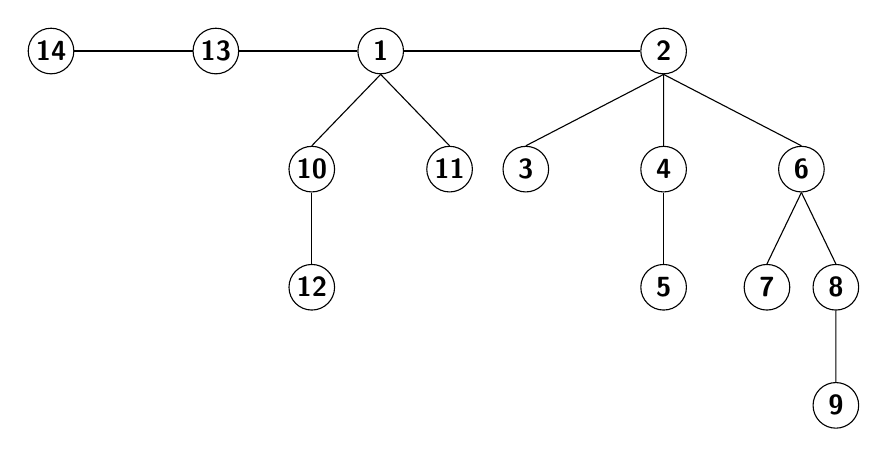
\begin{tikzpicture}[-,>=stealth',level/.style={sibling distance = 1.75cm/#1,level distance = 1.5cm}]
        \node [arn_n](A){14};
        \node [arn_n, right= 1.5cm of A](B){13};
        \node [arn_n, right= 1.5cm of B](C) {1}
            child{ node [arn_n] {10}
                    child{ node [arn_n] {12} 
                    }
        		}
        	child{ node [arn_n] {11}  }
        ;
        \node [arn_n, right= 3cm of C](D){2}
            child{ node [arn_n] {3}  }
            child{ node [arn_n] {4}
                    child{ node [arn_n] {5} 
                    }
        		}
        	child{ node [arn_n] {6}
                    child{ node [arn_n] {7} 
                    }
                    child{ node [arn_n] {8}
        							child{ node [arn_n] {9}}
                    }
        		}
        ;
        \draw (A) -- (B);
        \draw (B) -- (C);
        \draw (C) -- (D);
        \end{tikzpicture}
        \end{center}
    
    \end{enumerate}
\pagebreak    
\item
    \begin{enumerate}[label=(\alph*)]
        \item Edge List
        \\[\medskipamount]
            An edge list is essentially an array or pairs, in which each pair represents a connection between two nodes. This is simple to implement, but considering that the edges are not necessarily sorted, to find a particular edge requires a sequential search with a cost of \(O(n)\).
            
        \item Adjacency Matrix
        \\[\medskipamount]
            An adjacency matrix for \(n\) nodes is an \(n\:x\:n\) matrix, so the value at \((i,j)\) indicates whether a connection between nodes \(i\) and \(j\) exists. This makes looking up a connection a constant time problem, because we can directly navigate to the cell in the matrix. This requires much more space than a list, however, because you must also represent all connections, even if they don't exist.  
            
        \item Adjacency List
        \\[\medskipamount]
            The adjacency list combines aspects of the edge list and adjacency matrix to leverage the benefits each provides, look up time and conservation of memory. Here, each node is represented as an index in an array, and a list of all nodes it is connected to is stored at that index. Here, we still get nearly constant look up time, for we can simply navigate to the index in the array to look up the connections, and then just have to navigate through that list, making our operation in the worst case \(O(m)\) where \(m\) is the number of connections of the given node. This saves us space in respect to the matrix implementation, because instead of storing every possible connection, we simply store two times the amount of connections that exist. This is because each connection is recorded twice, once for each node in the connection.
            
    \end{enumerate}

\end{enumerate}
\end{document}